\documentclass[a4paper,french,bookmarks]{article}

\usepackage{./Structure/4PE18TEXTB}

\newboxans
\usepackage{booktabs}
\usepackage{tikz-3dplot}
 
\tdplotsetmaincoords{70}{122}

\begin{document}

    \renewcommand{\thesection}{\Roman{section}} 
    \renewcommand{\thesubsection}{\thesection.\Alph{subsection}}
    \setlist[enumerate]{font=\color{white5!60!black}\bfseries\sffamily}
    \renewcommand{\labelenumi}{\thesection.\arabic{enumi}.}
    \renewcommand*{\labelenumii}{\roman{enumii})}
    
    \newcommand{\ON}{\mathbf{ON}}
    
    \stylizeDocSpe{Physique}{Devoir maison n° 13}{}{Pour le mercredi 8 février 2023}
    
    \section{Premier problème}
    
    \begin{minipage}{0.3\linewidth}
        \resizebox{\linewidth}{!}{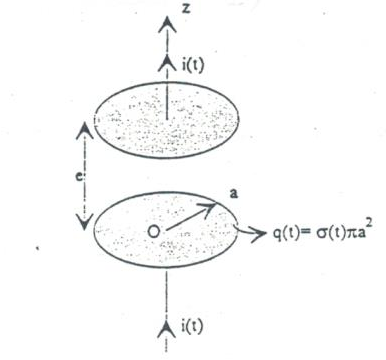
\includegraphics[]{dm13fig/dm13fig1.png}}
    \end{minipage}
    %
    \hfill
    %
    \begin{minipage}{0.6\linewidth}
        On considère un condensateur plan à armatures circulaires de rayon $a$, parfaitement conductrices, distantes de $e$, comme représenté sur la figure ci-contre.\bigskip
        
        A l'extérieur des armatures, un conducteur filiforme confondu avec l'axe $\p{Oz}$, parcouru par l'intensité $i\p{t}$, alimente le condensateur.\newline
        
        Sauf en question \enumrefraw{I.5}, on fera l'hypothèse de champ électrique $\vec{E_0}\p{t}$ uniforme entre les armatures, et nul à l'extérieur (l'espace inter-armatures est vide).
    \end{minipage}
    
    \begin{enumerate}
        \item Exprimer, en le justifiant, $\vec{E_0}\p{t}$ en fonction de $\sigma\p{t}$.
        
        \noafter
        %
        \boxans{
            On se place à de petites distances caractéristiques devant, $R$, de sorte que la situation soit similaire à celle d'un condensateur constitué de deux plans infinis, de densité surfacique de charge $\sigma\p{t}$ pour la plaque inférieure et de densité $-\sigma\p{t}$ pour la plaque supérieure. Par le cours, on a alors :
        }
        %
        \nobefore\yesafter
        %
        \boxansconc{
            \[ \vec{E_0}\p{t} = \dfrac{\sigma\p{t}}{\epsilon_0}\vec{e_z}\]
        }
        %
        \yesbefore
        
        \item En utilisant l'équation de \textsc{Maxwell-Ampère} sous forme intégrale, montrer qu'entre les armatures, le champ magnétique vaut :
        %
        \[ \vec{B_1}\p{r, t} = \dfrac{\mu_0 r \dot q}{2\pi a^2}\vec{e_\theta}\]
        
        \noafter
        %
        \boxans{
            D'après l'équation de \textsc{Maxwell-Ampère}, le champ entre les deux armatures circulaires vérifie : 
            %
            \[ \vec \nabla \wedge \vec{B_1} = \mu_0\p{\vec \jmath + \epsilon_0\dfrac{\partial \vec {E_0}}{\partial t}} \]
            %
            Il n'y a pas de courant, d'où $\vec \jmath = \vec 0$. Par ailleurs, $\dfrac{\partial \vec{E_0}}{\partial t} = \dfrac{1}{\epsilon_0}\dfrac{\dif \sigma}{\dif t}\vec{e_z} = \dfrac{1}{\epsilon_0\pi a^2}\dfrac{\dif q}{\dif t}\vec{e_z}$ donc :
            %
            \[ \vec \nabla \wedge \vec{B_1} = \dfrac{\mu_0\dot q}{\pi a^2}\vec{e_z}\]
            %
            Par ailleurs, la distribution de charges est symétrique au plan $\Pi_\text S\p{M, \vec{e_r}, \vec{e_z}}$, donc $\vec{B_1}\p{M} = B_\theta\p{M} \vec{e_\theta}$. En utilisant une formule du rotationnel en cylindrique, on obtient 
            %
            \[ \vec \nabla \wedge \vec{B_1} = \dfrac{1}{r}\dfrac{\partial \p{rB_\theta}}{\partial r}\vec{e_z} \qquad\text{donc}\qquad \dfrac{\partial \p{rB_\theta}}{\partial r} = \dfrac{\mu_0 r \dot q}{\pi a^2} \qquad\text{donc en primitivant}\qquad rB_\theta = \dfrac{\mu_0 r^2\dot q}{2\pi a^2} + C\]
        }
        %
        \nobefore\yesafter
        %
        \boxansconc{
            Par symétrie rotative en $r = 0$, on a $\vec{B_1}\p{r = 0} = \vec{0}$ d'où $C =0$. On a finalement bien $\vec{B_1}\p{r, t} = \dfrac{\mu_0r \dot q}{2\pi a^2}\vec{e_\theta}$.
        }
        %
        \yesbefore
        
        \item Lors de la décharge du condensateur, on a $q\p{t} = q_0e^{-\sfrac{t}{\tau}}$ Comparer alors $\omega_E = \dfrac{\epsilon_0}{2} E_0^2$ et $\omega_M = \dfrac{1}{2\mu_0}B_1^2$. Montrer en particulier que $\omega_M \ll \omega_E$ si $a \ll \lambda = c\tau$. Conclure.
        
        \noafter
        %
        \boxans{
            \[ \left\lbrace\begin{array}{lllll}
                \omega_E &= \dfrac{1}{2}\epsilon_0 {E_0}^2 &= \dfrac{\epsilon_0\sigma\p{t}^2}{2\epsilon_0^2} &= \dfrac{q\p{t}^2}{2\epsilon_0 \pi^2 a^4} &= \dfrac{q_0^2}{2\epsilon_0 \pi^2 a^4}e^{-2\sfrac{t}{\tau}}\\
                \omega_M &= \dfrac{1}{2\mu_0} {B_1}^2 &= \dfrac{\mu_0^2 r^2 \dot q^2}{2\mu_0 \times  2^2 \pi^2 a^4} &= \dfrac{\mu_0 r^2 \p{-\frac{q_0}{\tau}e^{-\sfrac{t}{\tau}}}^2}{8\pi^2 a^4} &= \dfrac{\mu_0 r^2 q_0^2}{8\pi^2 \tau^2 a^4}e^{-2\sfrac{t}{\tau}}
            \end{array}\right. \]
        }
        \nobefore
        %
        \boxansconc{
            On a donc $\dfrac{\omega_M}{\omega_E} = \dfrac{\epsilon_0\mu_0 r^2}{4 \tau^2} = \p{\dfrac{r}{\lambda}}^2$ et $r \leq a$ donc $a \ll \lambda$ d'où $\omega_M \ll \omega_E$. On remarquera que $\omega_\text{el}$ l'énergie du
        }
        %
        \yesbefore\yesafter
        %
        \boxansconc{
            champ électromagnétique vérifie $\omega_\text{el} = \omega_E + \omega_B$ donc $\omega_\text{el} \approx \omega_E$ : la majorité de cette énergie provient du champ électrique.
        }
        
        \item Calculer $\vec R$ pour $r = a$, puis le flux rentrant de $\vec R$ à l'intérieur du condensateur.
        
        \noafter
        %
        \boxans{
            \[ \vec R = \dfrac{\vec {E_1} \wedge \vec{B_1}\p{r = a}}{\mu_0} = \dfrac{\sigma a \dot q}{2\epsilon_0\pi a^2}\p{\vec{e_z} \wedge \vec{e_\theta}} = -\dfrac{\sigma \dot q}{2\epsilon_0\pi a}\vec{e_r}\]
            %
            On calcule le flux rentrant à l'intérieur du condensateur à l'aide de la surface correspondant à la paroi du cylindre entre les deux armatures, de vecteur surface $\vec \bcS = 2\pi a e \vec{e_r}$. On a donc :
            %
        }
        %
        \nobefore\yesafter
        %
        \boxansconc{
            \[ \Phi_\text{rentrant} = -\niint_{\bcS} \vec R \cdot \dif \vec \bcS = \dfrac{\sigma \dot q}{2\epsilon_0 \pi a} \niint \dif S = \dfrac{\sigma \dot q}{2\epsilon_0 \pi a}2\pi a e = \dfrac{e\sigma  \dot q}{\epsilon_0}\]
        }
        %
        \yesbefore
        
        \item On considère maintenant que le champ électrique entre les deux armatures n'est plus uniforme. On considère qu'il est de la forme :
        %
        \[ \vec E = E\p{r, t}\vec{e_z} \]
        %
        
        \begin{enumerate}
            \item À quelle équation aux dérivées partielles doit satisfaire $E\p{r, t}$ ?
            
            \item On montre que la solution de cette équation est une série, dont le premier terme est $\vec{E_0}\p{t}$ et dont on cherche ici à déterminer le deuxième terme $\vec{E_2}\p{r, t}$. En utilisant 
            
            \item On suppose de nouveau 
        \end{enumerate}
        
    \end{enumerate}
    
\end{document}